\documentclass{standalone}
\usepackage{tikz}
\usetikzlibrary{patterns, positioning}
\usepackage[sfdefault]{ClearSans} %% option 'sfdefault' activates Clear Sans as the default text font
\usepackage[T1]{fontenc}

\begin{document}
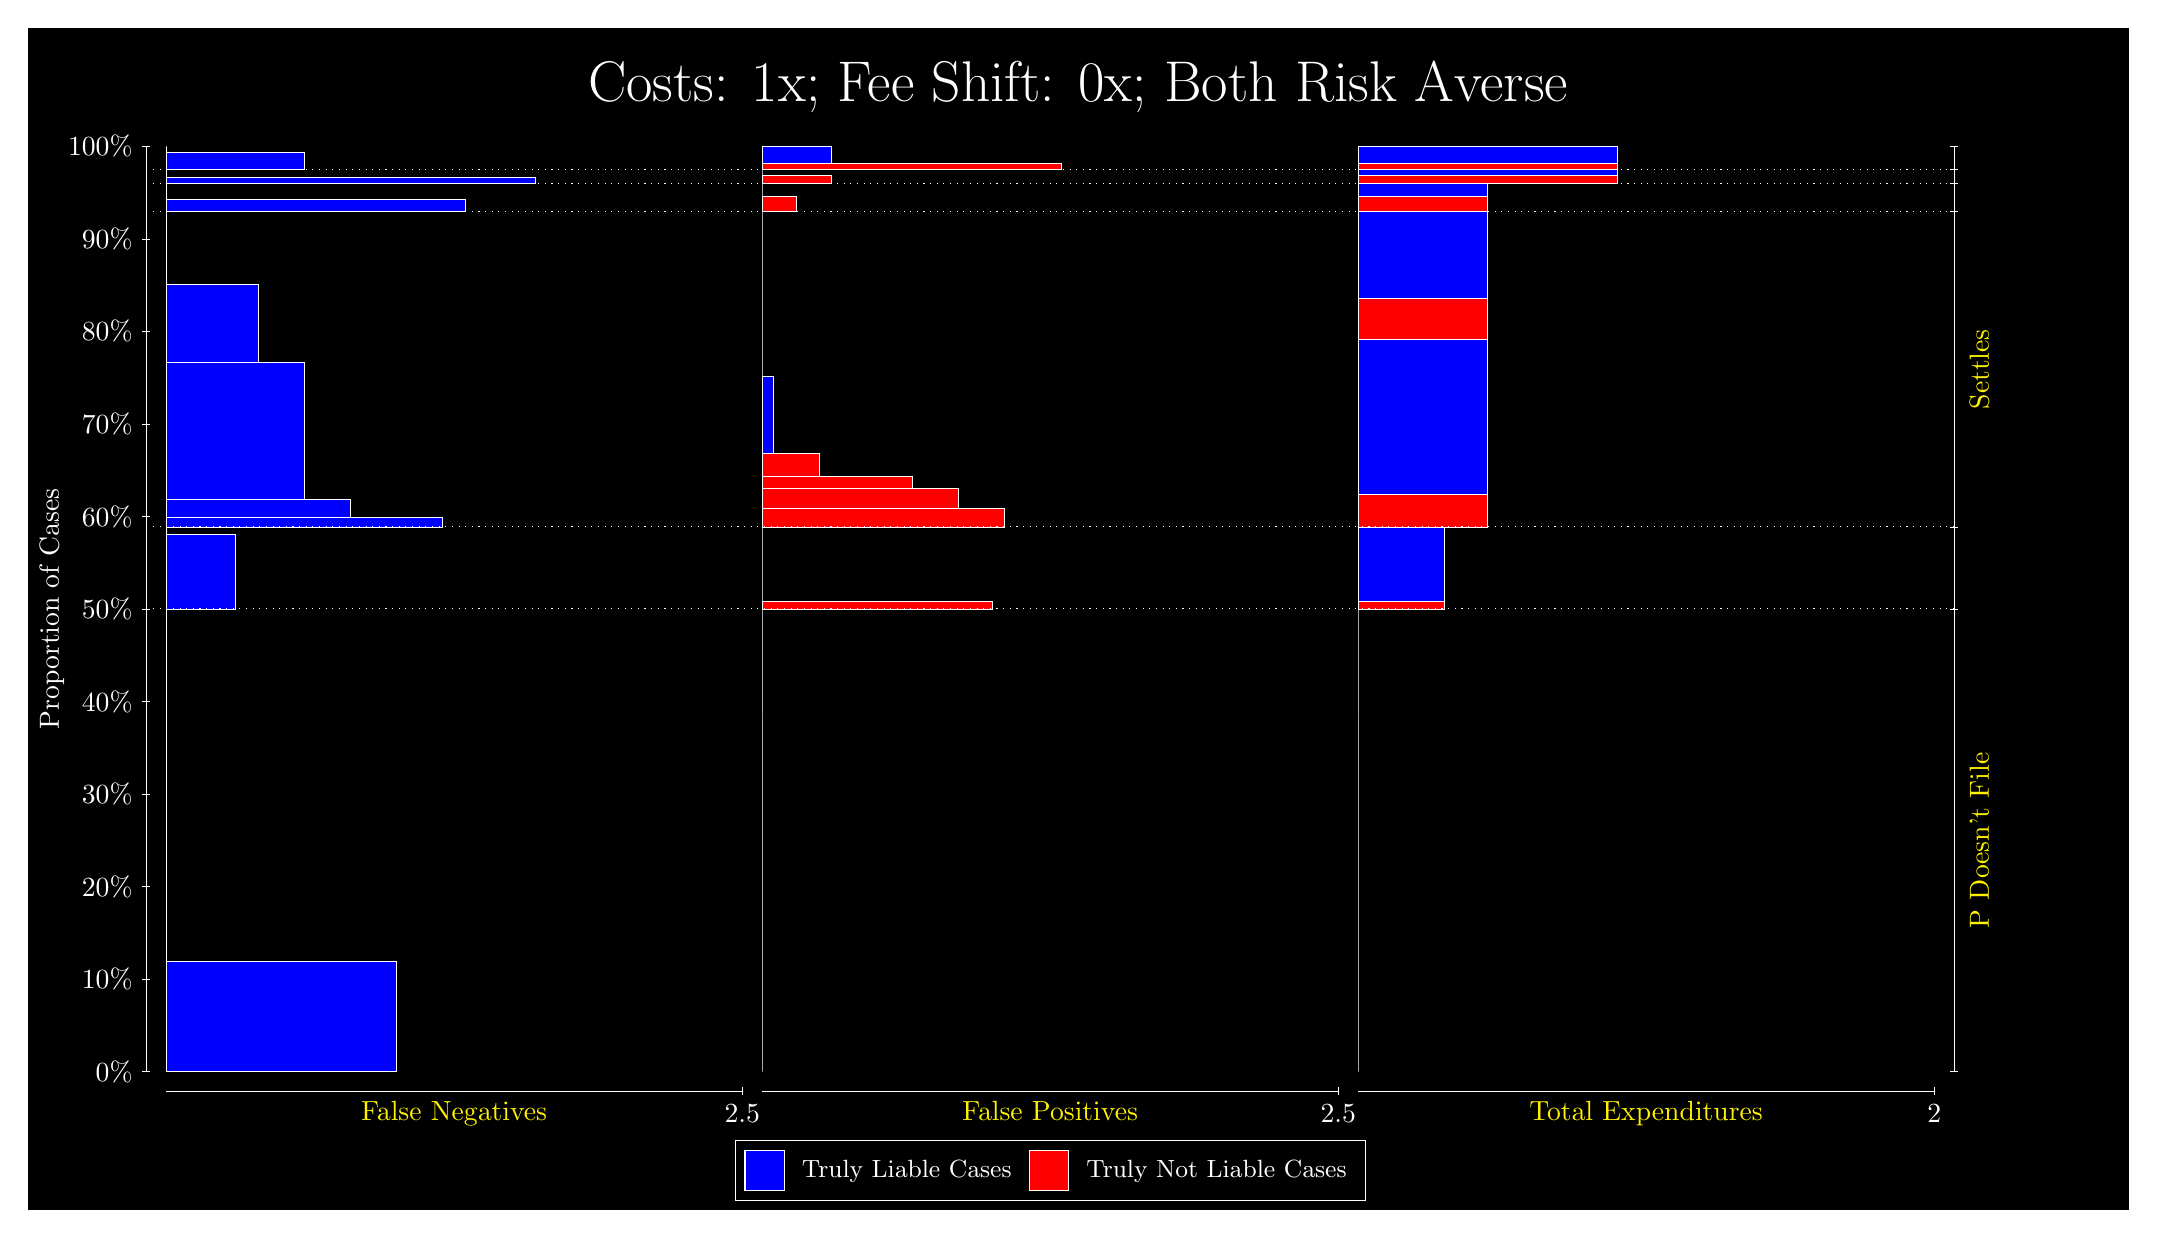
\begin{tikzpicture}
\draw[fill=black] (0,0) rectangle (26.667,15);
\draw[text=white] (0,13.5) rectangle (26.667,15) node[midway] {\huge Costs: 1x; Fee Shift: 0x; Both Risk Averse};
\draw[white, very thin] (1.5,1.75) -- (1.5,13.5);
\node[rotate=90, text=white, anchor=center] at (0.3, 7.625) {Proportion of Cases};
\draw[white, very thin] (1.45,1.75) -- (1.55,1.75);
\node[text=white, anchor=east] at (1.45, 1.75) {0\%};
\draw[white, very thin] (1.45,2.925) -- (1.55,2.925);
\node[text=white, anchor=east] at (1.45, 2.925) {10\%};
\draw[white, very thin] (1.45,4.1) -- (1.55,4.1);
\node[text=white, anchor=east] at (1.45, 4.1) {20\%};
\draw[white, very thin] (1.45,5.275) -- (1.55,5.275);
\node[text=white, anchor=east] at (1.45, 5.275) {30\%};
\draw[white, very thin] (1.45,6.45) -- (1.55,6.45);
\node[text=white, anchor=east] at (1.45, 6.45) {40\%};
\draw[white, very thin] (1.45,7.625) -- (1.55,7.625);
\node[text=white, anchor=east] at (1.45, 7.625) {50\%};
\draw[white, very thin] (1.45,8.8) -- (1.55,8.8);
\node[text=white, anchor=east] at (1.45, 8.8) {60\%};
\draw[white, very thin] (1.45,9.975) -- (1.55,9.975);
\node[text=white, anchor=east] at (1.45, 9.975) {70\%};
\draw[white, very thin] (1.45,11.15) -- (1.55,11.15);
\node[text=white, anchor=east] at (1.45, 11.15) {80\%};
\draw[white, very thin] (1.45,12.325) -- (1.55,12.325);
\node[text=white, anchor=east] at (1.45, 12.325) {90\%};
\draw[white, very thin] (1.45,13.5) -- (1.55,13.5);
\node[text=white, anchor=east] at (1.45, 13.5) {100\%};

\draw[white, very thin] (24.457,1.75) -- (24.457,13.5);
\draw[white, very thin] (24.407,1.75) -- (24.507,1.75);
\node[anchor=west] at (24.407, 1.75) {};
\draw[white, very thin] (24.407,7.6251) -- (24.507,7.6251);
\node[anchor=west] at (24.407, 7.6251) {};
\draw[white, very thin] (24.407,8.6672) -- (24.507,8.6672);
\node[anchor=west] at (24.407, 8.6672) {};
\draw[white, very thin] (24.407,12.673) -- (24.507,12.673);
\node[anchor=west] at (24.407, 12.673) {};
\draw[white, very thin] (24.407,13.027) -- (24.507,13.027);
\node[anchor=west] at (24.407, 13.027) {};
\draw[white, very thin] (24.407,13.206) -- (24.507,13.206);
\node[anchor=west] at (24.407, 13.206) {};
\draw[white, very thin] (24.407,13.5) -- (24.507,13.5);
\node[anchor=west] at (24.407, 13.5) {};

\draw[white, very thin, fill=blue] (1.75,1.75) rectangle (4.6775,3.1524);
\draw[white, very thin, fill=red] (1.75,3.1524) rectangle (1.75,7.6251);
\draw[white, very thin, fill=blue] (1.75,7.6251) rectangle (2.6283,8.5696);
\draw[white, very thin, fill=red] (1.75,8.5696) rectangle (1.75,8.6672);
\draw[white, very thin, fill=blue] (1.75,8.6672) rectangle (5.2631,8.7942);
\draw[white, very thin, fill=blue] (1.75,8.7942) rectangle (4.092,9.019);
\draw[white, very thin, fill=blue] (1.75,9.019) rectangle (3.5065,10.763);
\draw[white, very thin, fill=blue] (1.75,10.763) rectangle (2.921,11.744);
\draw[white, very thin, fill=red] (1.75,11.744) rectangle (1.75,12.673);
\draw[white, very thin, fill=blue] (1.75,12.673) rectangle (5.5558,12.83);
\draw[white, very thin, fill=red] (1.75,12.83) rectangle (1.75,13.027);
\draw[white, very thin, fill=blue] (1.75,13.027) rectangle (6.4341,13.102);
\draw[white, very thin, fill=red] (1.75,13.102) rectangle (1.75,13.206);
\draw[white, very thin, fill=blue] (1.75,13.206) rectangle (3.5065,13.424);
\draw[white, very thin, fill=red] (1.75,13.424) rectangle (1.75,13.5);
\draw[white, very thin, fill=red] (9.3189,1.75) rectangle (9.3189,6.2226);
\draw[white, very thin, fill=blue] (9.3189,6.2226) rectangle (9.3189,7.6251);
\draw[white, very thin, fill=red] (9.3189,7.6251) rectangle (12.246,7.7227);
\draw[white, very thin, fill=blue] (9.3189,7.7227) rectangle (9.3189,8.6672);
\draw[white, very thin, fill=red] (9.3189,8.6672) rectangle (12.393,8.8984);
\draw[white, very thin, fill=red] (9.3189,8.8984) rectangle (11.807,9.1617);
\draw[white, very thin, fill=red] (9.3189,9.1617) rectangle (11.222,9.308);
\draw[white, very thin, fill=red] (9.3189,9.308) rectangle (10.051,9.5957);
\draw[white, very thin, fill=blue] (9.3189,9.5957) rectangle (9.4652,10.577);
\draw[white, very thin, fill=blue] (9.3189,10.577) rectangle (9.3189,12.673);
\draw[white, very thin, fill=red] (9.3189,12.673) rectangle (9.758,12.87);
\draw[white, very thin, fill=blue] (9.3189,12.87) rectangle (9.3189,13.027);
\draw[white, very thin, fill=red] (9.3189,13.027) rectangle (10.197,13.131);
\draw[white, very thin, fill=blue] (9.3189,13.131) rectangle (9.3189,13.206);
\draw[white, very thin, fill=red] (9.3189,13.206) rectangle (13.125,13.282);
\draw[white, very thin, fill=blue] (9.3189,13.282) rectangle (10.197,13.5);
\draw[white, very thin, fill=red] (16.888,1.75) rectangle (16.888,6.2226);
\draw[white, very thin, fill=blue] (16.888,6.2226) rectangle (16.888,7.6251);
\draw[white, very thin, fill=red] (16.888,7.6251) rectangle (17.986,7.7227);
\draw[white, very thin, fill=blue] (16.888,7.7227) rectangle (17.986,8.6672);
\draw[white, very thin, fill=red] (16.888,8.6672) rectangle (18.534,9.0768);
\draw[white, very thin, fill=blue] (16.888,9.0768) rectangle (18.534,11.045);
\draw[white, very thin, fill=red] (16.888,11.045) rectangle (18.534,11.564);
\draw[white, very thin, fill=blue] (16.888,11.564) rectangle (18.534,12.673);
\draw[white, very thin, fill=red] (16.888,12.673) rectangle (18.534,12.87);
\draw[white, very thin, fill=blue] (16.888,12.87) rectangle (18.534,13.027);
\draw[white, very thin, fill=red] (16.888,13.027) rectangle (20.181,13.131);
\draw[white, very thin, fill=blue] (16.888,13.131) rectangle (20.181,13.206);
\draw[white, very thin, fill=red] (16.888,13.206) rectangle (20.181,13.282);
\draw[white, very thin, fill=blue] (16.888,13.282) rectangle (20.181,13.5);
\draw[white, dotted] (1.5,7.6251) -- (24.457,7.6251);
\draw[white, dotted] (1.5,8.6672) -- (24.457,8.6672);
\draw[white, dotted] (1.5,12.673) -- (24.457,12.673);
\draw[white, dotted] (1.5,13.027) -- (24.457,13.027);
\draw[white, dotted] (1.5,13.206) -- (24.457,13.206);
\draw[white, very thin] (1.75,1.5) -- (9.0689,1.5);
\node[text=yellow, anchor=north] at (5.4094, 1.5) {False Negatives};
\draw[white, very thin] (9.0689,1.45) -- (9.0689,1.55);
\node[text=white, anchor=north] at (9.0689, 1.45) {2.5};

\draw[white, very thin] (9.3189,1.5) -- (16.638,1.5);
\node[text=yellow, anchor=north] at (12.978, 1.5) {False Positives};
\draw[white, very thin] (16.638,1.45) -- (16.638,1.55);
\node[text=white, anchor=north] at (16.638, 1.45) {2.5};

\draw[white, very thin] (16.888,1.5) -- (24.207,1.5);
\node[text=yellow, anchor=north] at (20.547, 1.5) {Total Expenditures};
\draw[white, very thin] (24.207,1.45) -- (24.207,1.55);
\node[text=white, anchor=north] at (24.207, 1.45) {2};

\node[text=yellow, centered, rotate=90] at (24.777, 4.6875) {P Doesn't File};

\node[text=yellow, centered, rotate=90] at (24.777, 10.67) {Settles};




\draw (12.978300999999998,1.5) node[draw=none] (baseCoordinate) {};
\begin{scope}[align=center]
        \matrix[scale=0.5, draw=white, below=0.5cm of baseCoordinate, nodes={draw}, column sep=0.1cm]{
            \node[rectangle, draw, minimum width=0.5cm, minimum height=0.5cm, fill=blue] {}; &
            \node[draw=none, font=\small, text=white] (B) {Truly Liable Cases}; &
            \node[rectangle, draw, minimum width=0.5cm, minimum height=0.5cm, fill=red] {}; &
            \node[draw=none, font=\small, text=white] (B) {Truly Not Liable Cases}; \\
            };
\end{scope}

\end{tikzpicture}
\end{document}